\documentclass{standalone}
\usepackage{tikz}
\usetikzlibrary{patterns, positioning}


\begin{document}
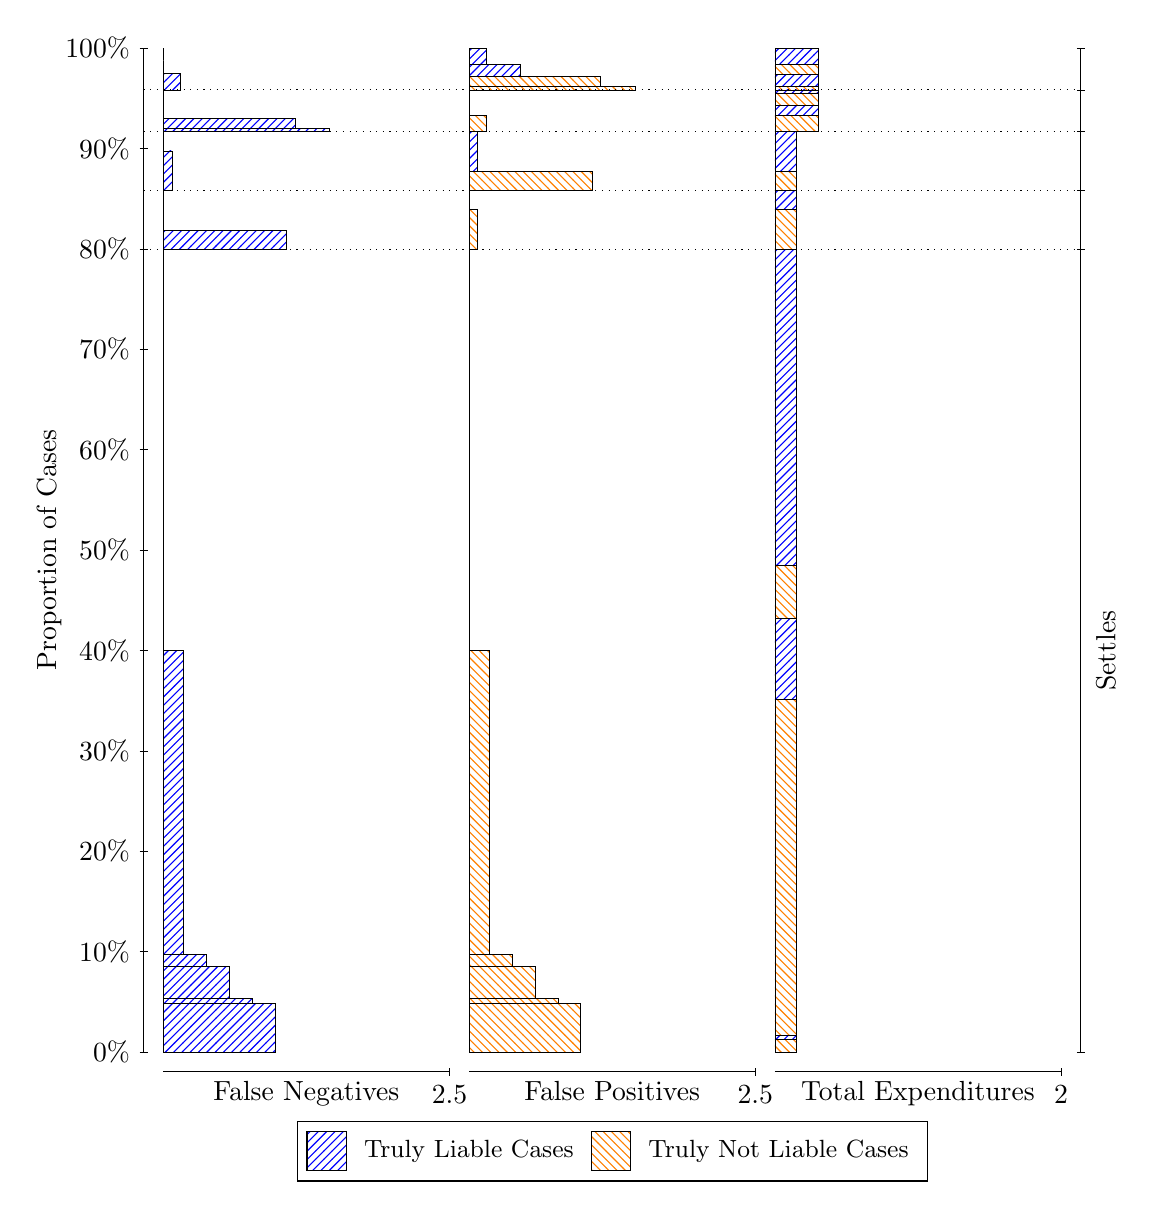
\begin{tikzpicture}
\draw[black, very thin] (1.5,1.75) -- (1.5,14.5);
\node[rotate=90, text=black, anchor=center] at (0.3, 8.125) {Proportion of Cases};
\draw[black, very thin] (1.45,1.75) -- (1.55,1.75);
\node[text=black, anchor=east] at (1.45, 1.75) {0\%};
\draw[black, very thin] (1.45,3.025) -- (1.55,3.025);
\node[text=black, anchor=east] at (1.45, 3.025) {10\%};
\draw[black, very thin] (1.45,4.3) -- (1.55,4.3);
\node[text=black, anchor=east] at (1.45, 4.3) {20\%};
\draw[black, very thin] (1.45,5.575) -- (1.55,5.575);
\node[text=black, anchor=east] at (1.45, 5.575) {30\%};
\draw[black, very thin] (1.45,6.85) -- (1.55,6.85);
\node[text=black, anchor=east] at (1.45, 6.85) {40\%};
\draw[black, very thin] (1.45,8.125) -- (1.55,8.125);
\node[text=black, anchor=east] at (1.45, 8.125) {50\%};
\draw[black, very thin] (1.45,9.4) -- (1.55,9.4);
\node[text=black, anchor=east] at (1.45, 9.4) {60\%};
\draw[black, very thin] (1.45,10.675) -- (1.55,10.675);
\node[text=black, anchor=east] at (1.45, 10.675) {70\%};
\draw[black, very thin] (1.45,11.95) -- (1.55,11.95);
\node[text=black, anchor=east] at (1.45, 11.95) {80\%};
\draw[black, very thin] (1.45,13.225) -- (1.55,13.225);
\node[text=black, anchor=east] at (1.45, 13.225) {90\%};
\draw[black, very thin] (1.45,14.5) -- (1.55,14.5);
\node[text=black, anchor=east] at (1.45, 14.5) {100\%};

\draw[black, very thin] (13.4,1.75) -- (13.4,14.5);
\draw[black, very thin] (13.35,1.75) -- (13.45,1.75);
\node[anchor=west] at (13.35, 1.75) {};
\draw[black, very thin] (13.35,11.944) -- (13.45,11.944);
\node[anchor=west] at (13.35, 11.944) {};
\draw[black, very thin] (13.35,12.69) -- (13.45,12.69);
\node[anchor=west] at (13.35, 12.69) {};
\draw[black, very thin] (13.35,13.437) -- (13.45,13.437);
\node[anchor=west] at (13.35, 13.437) {};
\draw[black, very thin] (13.35,13.969) -- (13.45,13.969);
\node[anchor=west] at (13.35, 13.969) {};
\draw[black, very thin] (13.35,14.5) -- (13.45,14.5);
\node[anchor=west] at (13.35, 14.5) {};

\draw[black, very thin, pattern color=blue, pattern=north east lines] (1.75,1.75) rectangle (3.167,2.368);
\draw[black, very thin, pattern color=blue, pattern=north east lines] (1.75,2.368) rectangle (2.8763,2.4283);
\draw[black, very thin, pattern color=blue, pattern=north east lines] (1.75,2.4283) rectangle (2.5857,2.8372);
\draw[black, very thin, pattern color=blue, pattern=north east lines] (1.75,2.8372) rectangle (2.295,2.9924);
\draw[black, very thin, pattern color=blue, pattern=north east lines] (1.75,2.9924) rectangle (2.0043,6.8467);
\draw[black, very thin, pattern color=orange, pattern=north west lines] (1.75,6.8467) rectangle (1.75,11.944);
\draw[black, very thin, pattern color=blue, pattern=north east lines] (1.75,11.944) rectangle (3.3123,12.187);
\draw[black, very thin, pattern color=orange, pattern=north west lines] (1.75,12.187) rectangle (1.75,12.69);
\draw[black, very thin, pattern color=blue, pattern=north east lines] (1.75,12.69) rectangle (1.859,13.194);
\draw[black, very thin, pattern color=orange, pattern=north west lines] (1.75,13.194) rectangle (1.75,13.437);
\draw[black, very thin, pattern color=blue, pattern=north east lines] (1.75,13.437) rectangle (3.8573,13.477);
\draw[black, very thin, pattern color=blue, pattern=north east lines] (1.75,13.477) rectangle (3.4213,13.607);
\draw[black, very thin, pattern color=orange, pattern=north west lines] (1.75,13.607) rectangle (1.75,13.969);
\draw[black, very thin, pattern color=blue, pattern=north east lines] (1.75,13.969) rectangle (1.968,14.175);
\draw[black, very thin, pattern color=orange, pattern=north west lines] (1.75,14.175) rectangle (1.75,14.344);
\draw[black, very thin, pattern color=blue, pattern=north east lines] (1.75,14.344) rectangle (1.75,14.5);
\draw[black, very thin, pattern color=orange, pattern=north west lines] (5.6333,1.75) rectangle (7.0503,2.368);
\draw[black, very thin, pattern color=orange, pattern=north west lines] (5.6333,2.368) rectangle (6.7597,2.4282);
\draw[black, very thin, pattern color=orange, pattern=north west lines] (5.6333,2.4282) rectangle (6.469,2.8371);
\draw[black, very thin, pattern color=orange, pattern=north west lines] (5.6333,2.8371) rectangle (6.1783,2.9923);
\draw[black, very thin, pattern color=orange, pattern=north west lines] (5.6333,2.9923) rectangle (5.8877,6.8469);
\draw[black, very thin, pattern color=blue, pattern=north east lines] (5.6333,6.8469) rectangle (5.6333,11.944);
\draw[black, very thin, pattern color=orange, pattern=north west lines] (5.6333,11.944) rectangle (5.7423,12.447);
\draw[black, very thin, pattern color=blue, pattern=north east lines] (5.6333,12.447) rectangle (5.6333,12.69);
\draw[black, very thin, pattern color=orange, pattern=north west lines] (5.6333,12.69) rectangle (7.1957,12.934);
\draw[black, very thin, pattern color=blue, pattern=north east lines] (5.6333,12.934) rectangle (5.7423,13.437);
\draw[black, very thin, pattern color=orange, pattern=north west lines] (5.6333,13.437) rectangle (5.8513,13.644);
\draw[black, very thin, pattern color=orange, pattern=north west lines] (5.6333,13.644) rectangle (5.6333,13.8);
\draw[black, very thin, pattern color=blue, pattern=north east lines] (5.6333,13.8) rectangle (5.6333,13.969);
\draw[black, very thin, pattern color=orange, pattern=north west lines] (5.6333,13.969) rectangle (7.7407,14.008);
\draw[black, very thin, pattern color=orange, pattern=north west lines] (5.6333,14.008) rectangle (7.3047,14.138);
\draw[black, very thin, pattern color=blue, pattern=north east lines] (5.6333,14.138) rectangle (6.2873,14.294);
\draw[black, very thin, pattern color=blue, pattern=north east lines] (5.6333,14.294) rectangle (5.8513,14.5);
\draw[black, very thin, pattern color=orange, pattern=north west lines] (9.5167,1.75) rectangle (9.7892,1.9052);
\draw[black, very thin, pattern color=blue, pattern=north east lines] (9.5167,1.9052) rectangle (9.7892,1.9654);
\draw[black, very thin, pattern color=orange, pattern=north west lines] (9.5167,1.9654) rectangle (9.7892,6.2289);
\draw[black, very thin, pattern color=blue, pattern=north east lines] (9.5167,6.2289) rectangle (9.7892,7.2559);
\draw[black, very thin, pattern color=orange, pattern=north west lines] (9.5167,7.2559) rectangle (9.7892,7.9341);
\draw[black, very thin, pattern color=blue, pattern=north east lines] (9.5167,7.9341) rectangle (9.7892,11.944);
\draw[black, very thin, pattern color=orange, pattern=north west lines] (9.5167,11.944) rectangle (9.7892,12.447);
\draw[black, very thin, pattern color=blue, pattern=north east lines] (9.5167,12.447) rectangle (9.7892,12.69);
\draw[black, very thin, pattern color=orange, pattern=north west lines] (9.5167,12.69) rectangle (9.7892,12.934);
\draw[black, very thin, pattern color=blue, pattern=north east lines] (9.5167,12.934) rectangle (9.7892,13.437);
\draw[black, very thin, pattern color=orange, pattern=north west lines] (9.5167,13.437) rectangle (10.062,13.644);
\draw[black, very thin, pattern color=blue, pattern=north east lines] (9.5167,13.644) rectangle (10.062,13.774);
\draw[black, very thin, pattern color=orange, pattern=north west lines] (9.5167,13.774) rectangle (10.062,13.93);
\draw[black, very thin, pattern color=blue, pattern=north east lines] (9.5167,13.93) rectangle (10.062,13.969);
\draw[black, very thin, pattern color=orange, pattern=north west lines] (9.5167,13.969) rectangle (10.062,14.008);
\draw[black, very thin, pattern color=blue, pattern=north east lines] (9.5167,14.008) rectangle (10.062,14.164);
\draw[black, very thin, pattern color=orange, pattern=north west lines] (9.5167,14.164) rectangle (10.062,14.294);
\draw[black, very thin, pattern color=blue, pattern=north east lines] (9.5167,14.294) rectangle (10.062,14.5);
\draw[black, dotted] (1.5,11.944) -- (13.4,11.944);
\draw[black, dotted] (1.5,12.69) -- (13.4,12.69);
\draw[black, dotted] (1.5,13.437) -- (13.4,13.437);
\draw[black, dotted] (1.5,13.969) -- (13.4,13.969);
\draw[black, very thin] (1.75,1.5) -- (5.3833,1.5);
\node[text=black, anchor=north] at (3.5667, 1.5) {False Negatives};
\draw[black, very thin] (5.3833,1.45) -- (5.3833,1.55);
\node[text=black, anchor=north] at (5.3833, 1.45) {2.5};

\draw[black, very thin] (5.6333,1.5) -- (9.2667,1.5);
\node[text=black, anchor=north] at (7.45, 1.5) {False Positives};
\draw[black, very thin] (9.2667,1.45) -- (9.2667,1.55);
\node[text=black, anchor=north] at (9.2667, 1.45) {2.5};

\draw[black, very thin] (9.5167,1.5) -- (13.15,1.5);
\node[text=black, anchor=north] at (11.333, 1.5) {Total Expenditures};
\draw[black, very thin] (13.15,1.45) -- (13.15,1.55);
\node[text=black, anchor=north] at (13.15, 1.45) {2};

\node[text=black, centered, rotate=90] at (13.72, 6.8468) {Settles};





\draw (7.449999999999999,1.5) node[draw=none] (baseCoordinate) {};
\begin{scope}[align=center]
        \matrix[scale=0.5, draw=black, below=0.5cm of baseCoordinate, nodes={draw}, column sep=0.1cm]{
            \node[rectangle, draw, minimum width=0.5cm, minimum height=0.5cm, pattern color=blue, pattern=north east lines] {}; &
            \node[draw=none, font=\small, text=black] (B) {Truly Liable Cases}; &
            \node[rectangle, draw, minimum width=0.5cm, minimum height=0.5cm, pattern color=orange, pattern=north west lines] {}; &
            \node[draw=none, font=\small, text=black] (B) {Truly Not Liable Cases}; \\
            };
\end{scope}

\end{tikzpicture}
\end{document}